%\VignetteIndexEntry{Portfolio Optimization in parma}
%\VignetteKeywords{portfolio, optimization, finance}
%\VignettePackage{parma}
\documentclass[11pt,a4paper]{article}
\usepackage[utf8]{inputenc}
\usepackage{amsmath}
\usepackage{amssymb}
\usepackage{anysize}
\usepackage{amsfonts}
\usepackage{lscape}
\usepackage{tabularx}
\usepackage{ctable}
\usepackage{subfig}
\usepackage{hyperref}
\usepackage{color}
\usepackage{harvard}
\usepackage{xkeyval}
\usepackage{listings}
\definecolor{sh_comment}{rgb}{0.12, 0.38, 0.18 } %adjusted, in Eclipse: {0.25, 0.42, 0.30 } = #3F6A4D
\definecolor{sh_keyword}{rgb}{0.37, 0.08, 0.25}  % #5F1441
\definecolor{sh_string}{rgb}{0.06, 0.10, 0.98} % #101AF9
\definecolor{lightgrey}{rgb}{0.94,0.94,0.94}
\lstset{ %
  basicstyle=\footnotesize\ttfamily,           % the size of the fonts that are used for the code
  numbers=left,                   % where to put the line-numbers
  numberstyle=\tiny\color{gray},  % the style that is used for the line-numbers
  stepnumber=0,                   % the step between two line-numbers. If it's 1, each line
  numbersep=5pt,                  % how far the line-numbers are from the code
  backgroundcolor=\color{white},      % choose the background color. You must add \usepackage{color}
  showspaces=false,               % show spaces adding particular underscores
  showstringspaces=false,         % underline spaces within strings
  showtabs=false,                 % show tabs within strings adding particular underscores
  frame=false,                   % adds a frame around the code
  rulecolor=\color{lightgrey},        % if not set, the frame-color may be changed on line-breaks within not-black text (e.g. commens (green here))
  tabsize=1,                      % sets default tabsize to 2 spaces
  captionpos=b,                   % sets the caption-position to bottom
  breaklines=true,                % sets automatic line breaking
  breakatwhitespace=false,        % sets if automatic breaks should only happen at whitespace
  title=\lstname,                   % show the filename of files included with \lstinputlisting;
  keywordstyle=\color{sh_keyword},          % keyword style
  commentstyle=\color{sh_comment},       % comment style
  stringstyle=\color{sh_string},         % string literal style
  morecomment=[l]{\#},
  morestring=[b]",
  morekeywords={show, round, weights, NULL, data, TRUE, FALSE, function, list, paste, args} % if you want to add more keywords to the set
}
%\marginsize{2cm}{2cm}{1cm}{1cm}
%\setlength{\textwidth}{16cm}
%\setlength{\oddsidemargin}{0cm}
%\setlength{\textheight}{24cm}
%\setlength{\headheight}{2cm}
\newtheorem{proof}{Proof}
\bibliographystyle{econometrica}
%\usepackage{Sweave}
\usepackage{graphicx}
\begin{document}
\title{Portfolio Optimization in \textbf{parma}}
\author{Alexios Ghalanos}
\date{\today}
\maketitle
\begin{abstract}
The \textbf{p}ortfolio \textbf{a}llocation and \textbf{r}isk \textbf{m}anagement 
\textbf{a}pplications (\textbf{parma}) package provides a set of models and 
methods for use in the allocation and management of capital in financial portfolios. 
It uniquely represents certain discontinuous problems using their smooth approximation 
counterparts and implements fractional based programming for the direct optimization 
of risk-to-reward ratios. This paper forms an introduction to the models and methods.
\end{abstract}
\clearpage
%\tableofcontents
\newpage
\section{Introduction}
Generally speaking, the portfolio management life-cycle is the process of
allocating and managing investment capital with respect to a set of
assumptions on the market dynamics and available universe of investable
assets. The assumptions made in the model building stage will generally
guide decisions on allocation, while trading and monitoring those
allocations forms part of risk management. Figure \ref{fig:mam}
succinctly illustrates the decision making process of model builing,
allocation and management (\emph{MAM}).\\
\begin{figure}[!ht]
\centering
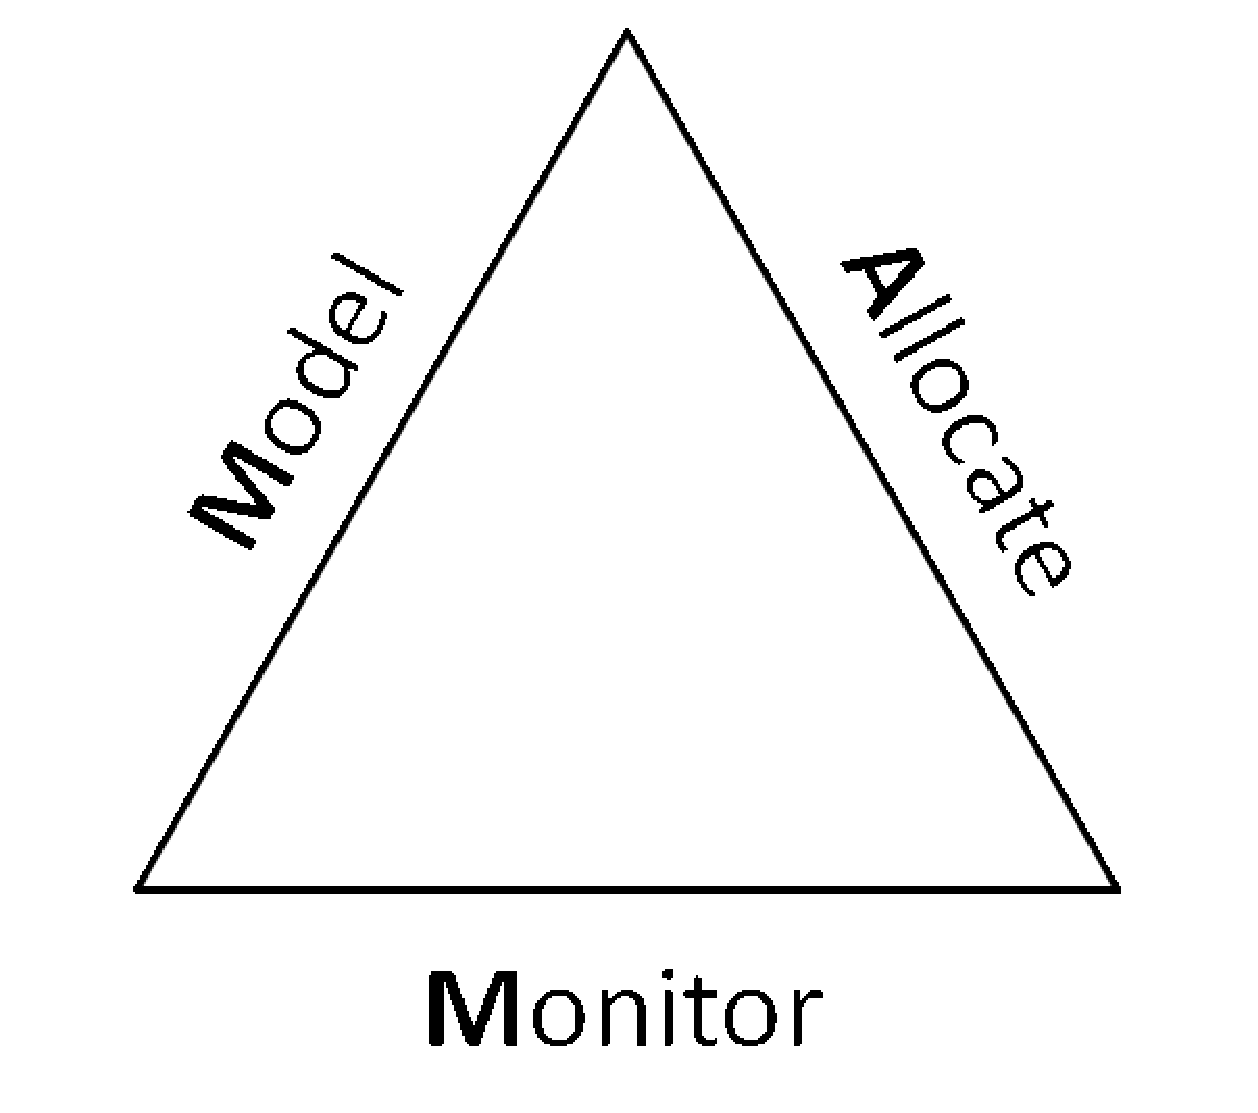
\includegraphics[scale=0.3]{mam.eps}
\caption[MAM's the word]{MAM's the word}\label{fig:mam}
\end{figure}

The \textbf{p}ortfolio \textbf{a}llocation and \textbf{r}isk
\textbf{m}anagement \textbf{a}pplications (\textbf{parma})
package provides a rich subset of models and methods for use in the
portfolio allocation process. The models are classified according to
the problem\textbackslash program class they belong to, namely
Linear \emph{LP}, Mixed Integer LP (\emph{MILP}), Quadratic (\emph{QP}),
Mixed Integer QP (\emph{MIQP}), Quadratically Constrained QP (\emph{QCQP}),
Non-Linear Convex (\emph{NLP}), Mixed Integer NLP (\emph{MINLP}) and
Non-Linear Non-Convex (\emph{GNLP}), the latter belonging to the
Global Optimization (\emph{GO}) type of problems.
Membership in these general problem classes is determined by the intersection
of the objective and constraint function space. Table \ref{table:solvers}
summarizes the types of problems currently supported in the \textbf{parma} package
which is completely dependent on the availability of high quality solvers of the
given types in R.
{\tiny
\ctable[
pos = h,
cap     = {Problems and Solvers in the \textbf{parma} package.},
caption = {Problems and Solvers in the \textbf{parma} package.},
label   = {table:solvers},
center
]
{lcccccccc}
{
\tnote[]{\tiny {\bf Note:} The Table presents the types of problems which the \textbf{parma} package can solve based on the available solvers,  where
\emph{T} means that a problem can be solved by the particular solver/type, \emph{F} that there is currently no available solver for this type of problem,
and \emph{TBI} that a solver will be implemented for that particular problem in due course. Note that for the scenario based optimization, all risk measures
which can be represented (without additional restrictions) as LP can also be represented as NLP,  with the exception of Conditional Drawdown at Risk for
which only an LP formulation exists. The covariance based optimization refers to the EV model which may also be solved using a scenario model as NLP.
\LL}
}{
\FL
\begin{tabular*}{1\textwidth}{@{\extracolsep{\fill}}lcccccccc}
\textbf{Problem Type} & \textbf{LP} & \textbf{MILP} & \textbf{QP} & \textbf{MIQP} & \textbf{QCQP} & \textbf{NLP} & \textbf{MINLP} & \textbf{GNLP} \\
\textbf{Solver} & \textbf{Rglpk} & \textbf{Rglpk} & \textbf{quadprog} & \textbf{.} & \textbf{Rsocp} & \textbf{nloptr} & \textbf{.} & \textbf{cmaes/crs} \\
\midrule  \relax
\textbf{Scenario [minrisk]} & T     & T     & .     & .     & .     & T     & .     & T \\ \relax
+    LP custom constraints & T     & .     & .     & .     & .     & .     & .     & . \\ \relax
+ NLP custom constraints & .     & .     & .     & .     & .     & T     & .     & T \\   \relax
+   cardinality constraints & .     & T     & .     & .     & .     & .     & TBI   & T \\ \relax
\textbf{Scenario optrisk} & T     & .     & .     & .     & .     & T     & .     & T \\ \relax
+    LP custom constraints & T     & .     & .     & .     & .     & .     & .     & . \\ \relax
+ NLP custom constraints & .     & .     & .     & .     & .     & T     & .     & T \\ \relax
+   cardinality constraints & .     & .     & .     & .     & .     & .     & .     & T \\ \relax
\textbf{Covariance minrisk} & .     & .     & T     & .     & .     & .     & .     & . \\ \relax
+  LP custom constraints & .     & .     & T     & .     & .     & .     & .     & . \\ \relax
+   Q custom constraints & .     & .     & .     & .     & TBI   & .     & .     & . \\ \relax
+ cardinality constraints & .     & .     & .     & F     & .     & .     & .     & . \\ \relax
\textbf{Covariance optrisk} & .     & .     & T     & .     & .     & .     & .     & . \\ \relax
+  LP custom constraints & .     & .     & T     & .     & .     & .     & .     & . \\ \relax
+   Q custom constraints & .     & .     & .     & .     & .     & .     & .     & . \\ \relax
+ cardinality constraints & .     & .     & .     & .     & .     & .     & .     & . \\ \relax
\end{tabular*}
\LL
}}

A range of popular risk measures are implemented, with the ability to perform
both risk minimization or optimal risk-reward optimization using fractional
programming methods. The package makes use of smooth approximations to
discontinuous functions to represent risk measures such as CVaR and LPM, as
well as leverage in long-short optimization, as proper convex and continuous
NLP problems, making use of analytic gradients for consistent and confident
solutions. For problems which cannot be represented as convex NLPs,
experimental support for global optimization is provided using derivative
free penalty functions but it is up to the user to decide how optimal such an
approach is. Serious users of GNLP problems should consider plugging in their
own high quality global optimization solvers the majority of which are either
non GPL or reside in another language\footnote{As a first attempt at
providing a reasonable Global solver for such problems, a ported (from
Matlab) version of the cmaes solver of \citet{Hansen2006} is made
available in this package with a rather comprehensive set of control
options.}. \\
Finally, a separate set of functions is also included for utility maximization
based on a Taylor Series expansion, taking as inputs moment and
co-moment matrices.\\
This document is organized as follows: Section \ref{sec:1} briefly discusses
the scenario approach to decision making in the context of stochastic
programming. Section \ref{sec:2} presents and discusses the risk measures
implemented in the package, and some recent topics in the definitions and
properties these measures. Section \ref{sec:3} discusses fractional
programming and the derivation of the optimal risk-reward portfolios. Section
\ref{sec:4} presents details of the implementation of the models in the parma
package, with a particular focus on the smooth approximations used, and
Section \ref{sec:5} a small FAQ section. Examples and demos may be found
online at:\\
 \url{http://www.unstarched.net/r-examples/parma/}.\\

The package is provided AS IS, without any implied warranty as to its accuracy
or suitability. A lot of time and effort has gone into the development of this
package, and it is offered under the GPL-3 license in the spirit of open
knowledge sharing and dissemination. If you do use the model in published work
DO remember to citet the package and author (type \textbf{citation("parma")} for
the appropriate BibTeX entry).

\section{Uncertainty and Scenario Based Allocation}\label{sec:1}
Randomness in the underlying environment leads to uncertainty, which can be
characterized, albeit approximately, by a model with a probability
distribution. The uncertainty is by no means resolved, but simply structured
under a set of assumptions for enabling decision making, by assigning some
probability to some 'unknowns' so that they become 'known unknowns'. The
purpose of stochastic programming (SP) is to incorporate such uncertainty
into the objective or constraint functions with a view to obtaining an
optimal set of decisions. This is done by constructing a scenario, or set of
scenarios, representing the possible future path or paths of the underlying
process (as a discrete time approximation to the continuous case)
incorporating the uncertainty with respect to the model and future, and from
which decisions can be based. These types of models were originally proposed
and analyzed among others by \citeauthor{Dantzig1956} (\citeyear{Dantzig1956},
\citeyear{Dantzig1992}), \citet{Beale1955}, \citet{Dantzig1993},
\citet{Madansky1962} and \citet{Charnes1959}. An excellent
exposition of SP models in asset and liability management can be found in
\citet{Kouwenberg2006}. Generally speaking, stochastic programming
covers a spectrum of uncertainty from that of complete information
(distribution model) to no information (anticipative model), with partial
information allowing for adaptation and multistage models with recourse. In
the \textbf{parma} package, only single stage anticipative models are
considered at present taking as inputs 1-period ahead scenarios of the
simulated discrete approximation to the multivariate conditional density.
For this purpose, the \emph{fscenario} function in the \textbf{rmgarch}
package provides for a set of parametric data generating processes from which
it is possible to generate such scenarios quite easily, as illustrated below:\\
\newline
\begin{Schunk}
\begin{Sinput}
> require(rmgarch)
> args(fscenario)
\end{Sinput}
\begin{Soutput}
function (Data, sim=1000, roll=0,
    model=c("gogarch", "dcc","cgarch", "var", "mdist"), spec=NULL,
    var.model=list(lag=1,lag.max=NULL,
        lag.criterion=c("AIC", "HQ", "SC", "FPE"), robust=FALSE,
        robust.control=list(gamma=0.25, delta=0.01, nc=10, ns=500)),
    mdist.model=list(distribution=c("mvn","mvt", "manig"), AR=TRUE, lag=1),
    spd.control=list(lower=0.1,upper=0.9, type="pwm", kernel="epanech"),
    cov.method=c("ML", "LW", "EWMA", "MVE", "MCD", "MVT", "BS"),
    cov.options=list(shrinkage=-1, lambda=0.96), solver="solnp",
    solver.control=list(), fit.control=list(eval.se=FALSE),
    cluster=NULL, save.output=FALSE, save.dir=getwd(),
    save.name=paste("S", sample(1:1000,1), sep=""), rseed=NULL, ...)
\end{Soutput}
\end{Schunk}
The models currently supported, are the 3 multivariate GARCH models GO-GARCH,
DCC and GARCH-Copula (DCC or non dynamic based) and the Vector AR model with
optional choice the type of covariance matrix used (\emph{cov.method}) for
the generation of the conditional multivariate random Normal errors in the
scenario. The choice of non dynamic multivariate distribution (\emph{mdist})
is not yet implemented. The option for parallel processing is provided by
passing a pre-created cluster object from the parallel package, and the replication
of results by passing seeding values (\emph{rseed}) to the random number
generator (either a single integer or a vector of integers of length roll+1).
In addition, the scenarios which may span several thousand rows and include rolling
simulated forecasts of the  conditional multivariate density (useful in backtesting)
can optionally be saved to file instead of being returned to the workspace,
where the function \emph{goload} reconstitutes previously saved data with
an object from such an operation. In addition to the scenario based mechanism,
the \textbf{fmoments} function generates conditional moment based forecasts
from the GO-GARCH and DCC models for use in the quadratic mean-variance (EV)
model as well as a separate function which maximizes utility based on a
Taylor series approximation of CARA (\emph{parmautility}), for which it
is possible to use, beyond the mean and covariance, higher co-moment tensors
generated from the GO-GARCH with maNIG (or the more general maGH) distribution.
\newline
\begin{Schunk}
\begin{Sinput}
> args(fmoments)
\end{Sinput}
\begin{Soutput}
function (spec, Data, n.ahead=1, roll=0, solver="solnp",
    solver.control=list(), fit.control=list(eval.se=FALSE),
    cluster=NULL, save.output=FALSE, save.dir=getwd(),
    save.name=paste("M", sample(1:1000, 1), sep=""), ...)
\end{Soutput}
\end{Schunk}
Scenarios or moments, whether they are derived from these auxiliary \textbf{rmgarch}
wrapper functions or a user's own programs, then form part of the \textbf{parmaspec}
function which defines the type of problem to be optimized:\\
\begin{Schunk}
\begin{Sinput}
> args(parmaspec)
\end{Sinput}
\begin{Soutput}
function (scenario=NULL, S=NULL, benchmark=NULL, benchmarkS=NULL,
    forecast=NULL, target=NULL, targetType=c("inequality", "equality"),
    risk=c("MAD", "MiniMax", "CVaR", "CDaR", "EV","LPM", "LPMUPM"),
    riskType=c("minrisk", "optimal"),
    options=list(alpha=0.05, threshold=999, moment=1), LB=NULL, UB=NULL,
    budget=1, leverage=NULL, ineqfun=NULL, ineqgrad=NULL, eqfun=NULL,
    eqgrad=NULL, uservars=list(), ineq.mat=NULL, ineq.LB=NULL, ineq.UB=NULL,
    eq.mat=NULL, eqB=NULL, max.pos=NULL, asset.names=NULL, ...)
\end{Soutput}
\end{Schunk}
The function consists of the data inputs: either a scenario or covariance
matrix and related optional benchmark details (for benchmark relative optimization),
the forecast and optionally portfolio target and whether this should be a
hard equality or inequality, the risk measure and optimization method,
and remaining arguments relating to the constraints. Note that NLP based
constraints in the \textbf{parma} package need to conform to a certain form,
an example of which is available in the \emph{parma.tests} folder, and in order for
the problems to remain  convex the inequality must be convex and the equality affine.
Departures from  these guidelines means that you are not guaranteed a global optimum.
More details can be found in the documentation and the online examples, whilst the types of
risk/deviation measures supported and their implementation are described in the next section.
\section{Risk and Deviation Measures}\label{sec:2}
In portfolio and resource allocation, characterization of the future
uncertainty  by a scenario of possible outcomes does not in itself provide
value to the decision maker unless he is able to rank, choose and allocate
among competing alternatives based on a set of preferences. Historically,
theories of such preferences have been normative, describing a certain set of
principles or axioms for rational behavior. The expected utility theory,
first proposed by \citet{Bernoulli1954} as a solution to the
St.Petersburg Paradox\footnote{Where the distinction between expected utility
and expected return was made.}, and formalized by \citet{VonNeumann1944}
into 4 key axioms (Completeness, Transitivity, Independence, Continuity),
provides the most popular approach\footnote{Though by no means the only
approach. See for example \citet{Savage1962} for subjective expected
utility, \citet{Quiggin1982} and \citet{Schmeidler1989} for rank
dependent utility and \citet{Zadeh1965} for Fuzzy Logic.} to rational
decision making. Risk attitudes in expected utility theory are usually
measured by the Arrow-Pratt (see \citet{Arrow1963}) definitions of
absolute and relative risk aversion (\emph{ARA} and \emph{RRA} respectively)
which are standardized measures of the degree of curvature in the utility
functions\footnote{ Formally, $ARA\left( W \right)= - \frac{{U''\left( W
\right)}}{{U'\left( W \right)}}$ and $RRA\left( W \right)= -
\frac{{WU''\left( W \right)}}{{U'\left( W \right)}}$.} Utility functions of
the form $U\left( W \right)= - \exp \left( { - \lambda W} \right)$, for
instance, have constant absolute risk aversion, which the \emph{paramutility}
function implements based on a 2 and 4 moment Taylor series approximation.\\
In an attempt to depart from the utility framework altogether and to make
use of criteria based on more objective and concrete concepts, a parallel
strand of research has focused mainly on the concept of loss aversion. A
first attempt at quantifying risk as the loss beyond a certain threshold was
the Safety-First criterion of \citet{Roy1952} which aimed at minimizing
the probability of being below an investor's minimum acceptable return
(\emph{MAR}). Later concepts have looked at improving on this measure by
penalizing losses below the threshold at different rates representing
different preferences. Irrespective of the type of measure, the more general
reward-risk approach has proved very popular both academically and in
practise since it enables preferences to be summarized in a few scalar
parameters such as the mean and variance. However, it was not until recently
that formal qualifications of the properties of such measures where defined
in seminal papers by \citet{Artzner1999} and \citet{Acerbi2002a} on
risk and \citet{Rockafellar2006} on deviation, with the latter
establishing the connection between the two and briefly described here.
Consider the probability space $\{\Omega, \mathcal{A}, P\}$ where $P$ is the
probability on the $\mathcal{A}$ measurable subsets of $\Omega$.
\citet{Rockafellar2006} defined a set of axioms which functions in the
linear space $\mathcal{L}^2$ (which include the mean and variance) should
satisfy. Formally, the deviation measure functionals
$\mathcal{D}:{\mathcal{L}^2}(\Omega) \to \left[ {0,\infty } \right]$ should
satisfy the following axioms:
\begin{itemize}
\item (D1) $\mathcal{D}\left(C\right)=0$ $\forall$ constants C,
\item (D2) $\mathcal{D}\left(\lambda X\right)=\lambda\mathcal{D}\left(X\right)$ $\forall$ X and $\lambda>0$,
\item (D3) $\mathcal{D}\left(X+X'\right)\leq \mathcal{D}\left(X\right)+\mathcal{D}\left(X'\right)$ $\forall$ X and $X'$,
\item (D4) $\mathcal{D}\left(X\right)\geq 0$ $\forall$ X and $\mathcal{D}\left(X\right)>0$ $\forall$ nonconstant X,
\end{itemize}
where (D1) is the translation invariance property under the special condition
given  for constants (i.e. insensitivity to constant shifts), (D2) represents
the positive homogeneity property, (D3) the subadditivity property , while
(D4) is the lower bound implied by the domain of $\mathcal{D}$.
\citet{Artzner1999} provides the equivalent 'coherent' risk measure
functionals $\mathcal{R}:{\mathcal{L}^2}(\Omega) \to \left( {-\infty,\infty }
\right]$ which should satisfy the following axioms:
\begin{itemize}
\item (R1) $\mathcal{R}\left(C\right)=-C$ $\forall$ constants C,
\item (R2) $\mathcal{R}\left(\lambda X\right)=\lambda\mathcal{R}\left(X\right)$ $\forall$ X and $\lambda>0$,
\item (R3) $\mathcal{R}\left(X+X'\right)\leq \mathcal{R}\left(X\right)+\mathcal{R}\left(X'\right)$ $\forall$ X and $X'$,
\item (R4) $\mathcal{R}\left(X\right)\leq \mathcal{R}\left(X'\right)$ whenever $X\geq X'$,
\end{itemize}
where (R1) is the translation invariance property, (R2) is positive
homogeneity, (R3) subadditivity property and (R4) the monotonicity property.
More plainly, (R1) implies that adding a constant to a set of losses does not
change the risk, (R2) that holdings and risk scale by the same linear factor,
(R3) that portfolio risk cannot be more than the combined risks of the
individual positions, and (R4) that larger losses equate to larger risks.
\citet{Acerbi2002a} defined the family of spectral risk measures as
those with weighted\footnote{With positive weights which are normalized to sum to 1.}
quantiles, possessing the properties of coherent risk measures and additionally:
\begin{itemize}
\item (R5) If $\mathcal{F}\left( X \right)=\mathcal{F}\left( Y \right)$, then $\mathcal{R}\left( X \right)=\mathcal{R}\left( Y \right)$,
\end{itemize}
which essentially implies that portfolios with equal cumulative distribution
functions ($\mathcal{F}$) should have the same risk.
\citet{Rockafellar2006} defined a one-to-one relationship between
deviation and risk measures\footnote{In the rest of this paper, I will refer
to 'risk' to mean both risk and deviation measures.} which satisfy properties
(R1),(R2),(R3) and are strictly expectation bounded so that
$\mathcal{R}(X)>E\left[-X\right]$ as:
\begin{itemize}
\item $\mathcal{D}\left( X \right)=\mathcal{R}\left( {X - E\left[ X \right]} \right)$,
\item $\mathcal{R}\left( X \right)=E\left[ { - X} \right] + \mathcal{D}\left( X \right)$.
\end{itemize}
In the following subsections, I consider the properties and representations
of 5 interesting and popular measures which are implemented in the
\textbf{parma} package . The first 3 loosely belong to the general $L^p$
function space\footnote{The $L^p$ function space is defined as:
\begin{equation}
{\left\| e \right\|_p}={\left( {\sum\limits_{j=1}^m {{{\left| {{e_j}} \right|}^p}} } \right)^{1/p}}
\end{equation}
with $p=1$ representing the absolute (or Manhattan distance) measure, $p=2$
the  standard deviation (or Euclidean distance) where we can make use of
variance instead because of the monotone transformation property, and
$p=\infty$ represents the largest absolute value where we can represent the
losses for Minimax optimization.} and include the Absolute Deviation,
Variance and Minimax measures, while the other 2 are the threshold based
measures of Lower Partial Moments (\emph{LPM}) and Conditional Value at Risk
(\emph{CVaR}).
\subsection{Mean Variance (EV)}
\citet{Markowitz1952} ushered in the era of modern portfolio management
with the introduction of the Mean-Variance model of risk-return. Variance is
a valid measure of risk for ranking preferences if either the investor
exhibits quadratic utility (in which case it does not matter whether the
underlying data is multivariate normal), or the underlying data is
multivariate normal (in which case the utility of the investor is irrelevant
since variance is the optimal choice). The optimization problem may be posed
as the following NLP problem:
\begin{equation}\label{mvnlp}
\begin{gathered}
  \mathop {\min }\limits_w \frac{1}{n}\sum\limits_{i=1}^n {{{\left( {\sum\limits_{j=1}^m {{w_j}\left( {{r_{i,j}} - {\mu _j}} \right)} } \right)}^2}}  \hfill \\
  s.t. \hfill \\
  \sum\limits_{j=1}^m {{w_j}{\mu _j}=C}  \hfill \\
  \sum\limits_{j=1}^m {{w_j}=1}  \hfill \\
  {w_j} \ge 0,\forall j \in \left\{ {1,\dots,m} \right\} \hfill \\
\end{gathered}
\end{equation}
where $w$ represent the weights of the $j=1,\dots,m$ assets, $i=1,\dots,n$
are the number of periods or scenario points for the returns $r$ and $\mu_j$
the forecast return. The problem effectively minimizes portfolio variance
subject to the portfolio forecast return being equal to $C$, a full
investment constraint and positivity constraints on the weights. While it is
simple to express the problem in its quadratic form such that variance is
equal to $w'\Sigma w$, I leave the problem in its more general NLP form which
admits nonlinear constraints which would for example include long-short
optimization with a leverage constraint.\footnote{In the case of quadratic
based constraints, the problem can also be posed as a second order cone
(\emph{SOCP}) problem which will be implemented in a future update to the
package.} Criticisms of variance as a valid method for ranking portfolios is
mainly aimed at the quadratic utility assumption which seems nothing more
than a mathematical convenience rather than a reflection of reality, leading
to the strange case of investors desiring less to more after a certain point
on the utility curve, whilst the multivariate normality assumption is not
usually borne out by the data. The symmetric nature of variance, penalizing
both up and down deviations at the same rate was criticized by quite early on
by \citet{Hanoch1969}\footnote{The criticism was in fact also aimed at
any symmetric dispersion measure, not just variance.}, while its lack of
consistency with stochastic dominance relations should have effectively
buried it as a method for portfolio allocation. However, its tractability and
ease of use has made it a very popular choice, particularly for the modelling
of monthly returns, with numerous extensions to provide for robustness and
uncertainty mainly in the derivation of the covariance matrix. For example
\citet{James1956} provide for a shrinkage estimator, \citet{Black1992} a
semi-Bayesian approach while \citet{Michaud1989} a general criticism of the
approach with a patented alternative based on resampling methods. The Vector AR
model in the package allows for a choice of covariance estimators to be chosen
for the simulation of the random scenario matrix.
\subsection{Mean Absolute Deviation (MAD)}
In the early days of computer programming, large scale quadratic problems
were computationally more demanding to solve than linear problems. In light
of this, \citet{Konno1991} introduced a piece-wise linear formulation of
the absolute deviation function as an alternative to the
\citet{Markowitz1952} method. The standard NLP objective function may be
formulated as:
\begin{equation}\label{madnlp}
\begin{gathered}
\frac{1}{n}\sum\limits_{i=1}^n {\left| {\sum\limits_{j=1}^m {{w_j}\left( {{r_{i,j}} - {\mu _j}} \right)} } \right|}
\end{gathered}
\end{equation}
which \citet{Konno1991} reduced to the following piece-wise linear problem:
\begin{equation}\label{madlp}
\begin{gathered}
  \mathop {\min }\limits_{w,d} \frac{1}{n}\sum\limits_{i=1}^n {{d_i}}  \hfill \\
  s.t. \hfill \\
  \sum\limits_{j=1}^m {\left( {{r_{i,j}} - {\mu _j}} \right){w_j} \leq {y_i},\forall i \in \left\{ {1,\dots,n} \right\}}  \hfill \\
  \sum\limits_{j=1}^m {\left( {{r_{i,j}} - {\mu _j}} \right){w_j} \geq  - {y_i},\forall i \in \left\{ {1,\dots,n} \right\}}  \hfill \\
  \sum\limits_{j=1}^m {{w_j}{\mu _j}=C}  \hfill \\
  \sum\limits_{j=1}^m {{w_j}=1}  \hfill \\
  {w_j} \geq 0,\forall j \in \left\{ {1,\dots,m} \right\} \hfill \\
\end{gathered}
\end{equation}
where $d$ represent the absolute deviations of the portfolio from its
forecast mean, forming a vector of variables of size $n$ (length of the
scenario) to be optimized. However, the constraints imposed to create the
piece-wise linear function for the absolute deviation requires two $n\times
n$ diagonal matrices stacked together\footnote{\citet{Feinstein1993}
provide for a reformulated representation with only one n diagonal matrix.}
which may lead to computer memory problems for very large scenarios. This is
in direct contrast to the EV model which only depends on the number of
assets. Furthermore, while in the EV model deviations from the mean are
penalized at an increasing rate arising from the square function, in the MAD
model deviations are penalized at a linear rate which may not realistically
represent the average investor. However, by not giving undue weight to the
extreme observations, the MAD model may be more robust to possible
misspecification in the dynamics from which the scenario was generated.
Extensions to the model have included the addition of skewness in
\citet{Konno1993}, and semi-absolute deviation first suggested by
\citet{Speranza1993} who showed that the mean semi-deviation is a half
of the mean absolute deviation from the mean. Similar to the EV model, the
MAD model lacks consistency with stochastic dominance relations.
\subsection{Minimizing Regret (MiniMax)}
The MiniMax model of \citet{Young1998a}, aims to minimize the maximum loss,
$\max \left( {\sum\limits_{j=1}^m {- {r_{i,j}}{w_j}} ,\forall i=1,\dots,n} \right)$
and as such is a very conservative criterion. It has a very simple LP formulation:
\begin{equation}\label{eq:minimax}
\begin{gathered}
  \mathop {\min }\limits_{{M_p},w} {M_p} \hfill \\
  s.t. \hfill \\
  {M_p} - \sum\limits_{j=1}^m {{w_j}} {r_{i,j}} \leq 0,\forall i=\left\{ {1,\dots,n} \right\} \hfill \\
  \sum\limits_{j=1}^m {{w_j}{\mu _j}=C}  \hfill \\
  \sum\limits_{j=1}^m {{w_j}=1}  \hfill \\
  {w_j} \geq 0,\forall j \in \left\{ {1,\dots,m} \right\} \hfill \\
\end{gathered}
\end{equation}
where $M_p$ is the objective minimization value representing the maximum loss
of the portfolio and guaranteed to be bounded from above by the maximum
portfolio loss as a result of the first constraint. While
\citet{Young1998a} only considered the problem in light of historical
scenarios, there is no reason why $r$ in the formulation may not represent a
future simulated forecast scenario. Contrary to the MAD model, it only
requires 1 additional variable and $n\times 1$ additional constraint vector
in the LP formulation, and as such does not pose any computational challenges
even for very large problems. The Minimax principle is also consistent with
expected utility theory at the limit based on a very risk averse decision
maker, and a good approximation to the EV model when returns are multivariate
Normal. Interestingly, the model is also a limiting case of the Conditional
Value at Risk spectral risk measure described in the Section \ref{cvar}.
\subsection{Lower Partial Moments (LPM)}\label{LPM}
The concept of penalizing deviations below a certain threshold at a different
rate is at the heart of modern risk management and was already hinted at by
\citet{Markowitz1952} in a reference to semi-standard deviation. This
was later formalized into a very general class of measures by
\citet{Stone1973}, and the Lower Partial Moment (\emph{LPM}) framework
of \citet{Fishburn1977} which, in the continuous case, may be defined
as:
\begin{equation}
LP{M_{a ,\tau }}\left( f \right)=\int\limits_{ - \infty }^\tau  {{{\left( {\tau  - x} \right)}^a }f\left( x \right)dx}
\end{equation}
where $a$ is some positive number which represents the rate at which deviations
below the threshold $\tau$ are penalized and $f$ some density function.
In the discrete case, the function may be represented as:
\begin{equation}
LP{M_{a ,\tau }}\left( x \right)=E\left[ {\max {{\left( {\tau  - x,0} \right)}^a}} \right].
\end{equation}
Upper Partial Moments (\emph{UPM}) are defined similarly. Usually, in the
portfolio optimization context, the measure is standardized by raising it to
the power of $\frac{1}{a}$. \citet{Fishburn1977} derived a utility
representation for this measure consistent with the von Neumann-Morgenstern
axioms, and represented as:
\begin{equation}\label{eq:lpmutility}
U\left( x \right)=\begin{array}{*{20}{c}}
   {x - {k}{{\left( {\tau  - x} \right)}^{{a_l}}}} & {x < \tau }  \\
   x & {x \geq \tau }  \\
\end{array}
\end{equation}
where $k$ is a positive constant. \citet{Harlow1989} describe an asset
pricing model in the mean-lower partial moment framework (MLPM) and show that
an MLPM framework is consistent with a very general set of utility functions.
For example, the hyperbolic absolute risk aversion (\emph{HARA}) class of
utility functions  is consistent with $1^{st}$-degree LPM, whereas any risk
averse utility function displaying skewness preference with positive first
and third derivatives and negative second derivatives are consistent with
$2^{nd}$-degree LPM. In addition to this strong link with expected utility
theory, \citet{Bawa1977}, \citet{Bawa1978} and
\citet{Fishburn1977} showed that stochastic dominance is equivalent to
all degrees
of n-degree LPM.\\
The portfolio optimization problem can be posed as follows:
\begin{equation}
\begin{gathered}
 {\min {{\left( {\frac{1}{n}\sum\limits_{i=1}^n {\max {{\left( {0,\tau  - \left( {\sum\limits_{j=1}^m {{w_j}{r_{j,i}}} } \right)} \right)}^a}} } \right)}^{1/a}}}  \hfill \\
  s.t. \hfill\\
  \sum\limits_{j=1}^m {{w_j}{\mu _j}=C}  \hfill \\
  \sum\limits_{j=1}^m {{w_j}=1}  \hfill \\
  {w_j} \geq 0,\forall j \in \left\{ {1,\dots,m} \right\} \hfill \\
\end{gathered}
\end{equation}
Special cases are $a=0$ representing the shortfall probability or
Safety-First  model of \citet{Roy1952}, $a=1$ the below target shortfall
and $a=2$ the shortfall variance which is equivalent to the central
semi-variance when $\tau=E\left(x\right)$. When $a=1$, an LP formulation
exists and is given by:
\begin{equation}
\begin{gathered}
  \mathop {\min }\limits_w \frac{1}{n}\sum\limits_{i=1}^n {{d_i}}  \hfill \\
  s.t. \hfill \\
  \tau  - \sum\limits_{j=1}^m {{w_j}{r_{j,i}}}  \leq {d_i},\forall i \in \left\{ {1,\dots,n} \right\} \hfill \\
  \sum\limits_{j=1}^m {{w_j}{\mu _j}=C}  \hfill \\
  \sum\limits_{j=1}^m {{w_j}=1}  \hfill \\
  {w_j} \geq 0,\forall j \in \left\{ {1,\dots,m} \right\} \hfill \\
  {d_i} \geq 0,\forall i \in \left\{ {1\dots,n} \right\} \hfill \\
\end{gathered}
\end{equation}
The \textbf{parma} package implements the general LPM as NLP, but also
includes  the  special case when $a=1$ as an LP formulation. For positive
values of $a$ other than 1, the discontinuous max function appears to pose
some problems in the optimization strategy. \citet{Nawrocki1989} devised
a heuristic measure which approximates the function using only quadratic
programming methods. Instead, I replace the max function with a smoothed
approximation for which derivatives exist and discussed further in Section
\ref{sec:4}. With regards to the choice of threshold variable $\tau$, the
choice may be motivated by the investor's minimum acceptable return, some
benchmark rate\footnote{However, \citeauthor{Brogan2005}
(\citeyear{Brogan2005}, \citeyear{Brogan2008}) have shown that for the
linear separation property to hold, which assumes convexity of the mean-LPM
space, the threshold must either be equal to the risk free rate or the mean
of the portfolio.} or any other reasonable choice. A simple choice which
makes use of the properties of this deviation measure is to use the mean of
the portfolio (this is implemented by passing threshold=999 in the options
to the \textbf{parmaspec} function) which is equivalently equal to using a
threshold of zero and passing a demeaned scenario matrix.\footnote{This is
because the following general relationship holds for LPM measures:
\begin{equation}\label{eq:lpmscaling1}
LP{M_{\tau ,a}}\left( X \right)=LP{M_{t + C,a}}\left( {X + C} \right).
\end{equation}
which is equivalent to property (D1) presented previously, when accounting
for the threshold parameter's shift by the constant $C$. Additionally, and
with important implications in fractional programming, the LPM measure also
has the scaling property so that:
\begin{equation}\label{eq:lpmscaling2}
LP{M_{\tau ,a}}\left( X \right)=\frac{1}{b}LP{M_{bt,a}}\left( {bX} \right),
\end{equation}
where it is understood that for the non-standardized version of the measure,
i.e. when not raised to the power of $\frac{1}{a}$, the measure is multiplied
not
by $\frac{1}{b}$ but $\frac{1}{b^a}$ instead.}\\
Because the linear reward function may be too restrictive in practise,
\citet{Holthausen1981} extended the LPM model to include a non-linear
reward measure so that for $x\geq\tau$ in \eqref{eq:lpmutility}
$U\left(x\right)=x + {\left( {x - \tau } \right)^{{a_u}}}$, where $a_u$ is
the power exponent for the upper partial moment, thus effectively capturing a
range of linear and nonlinear utility curves (such as S-shaped and inverse
S-shaped) with reference to gains and losses as illustrated in the example in
Figure \ref{fig:lpmutility}.
\begin{figure}
\centering
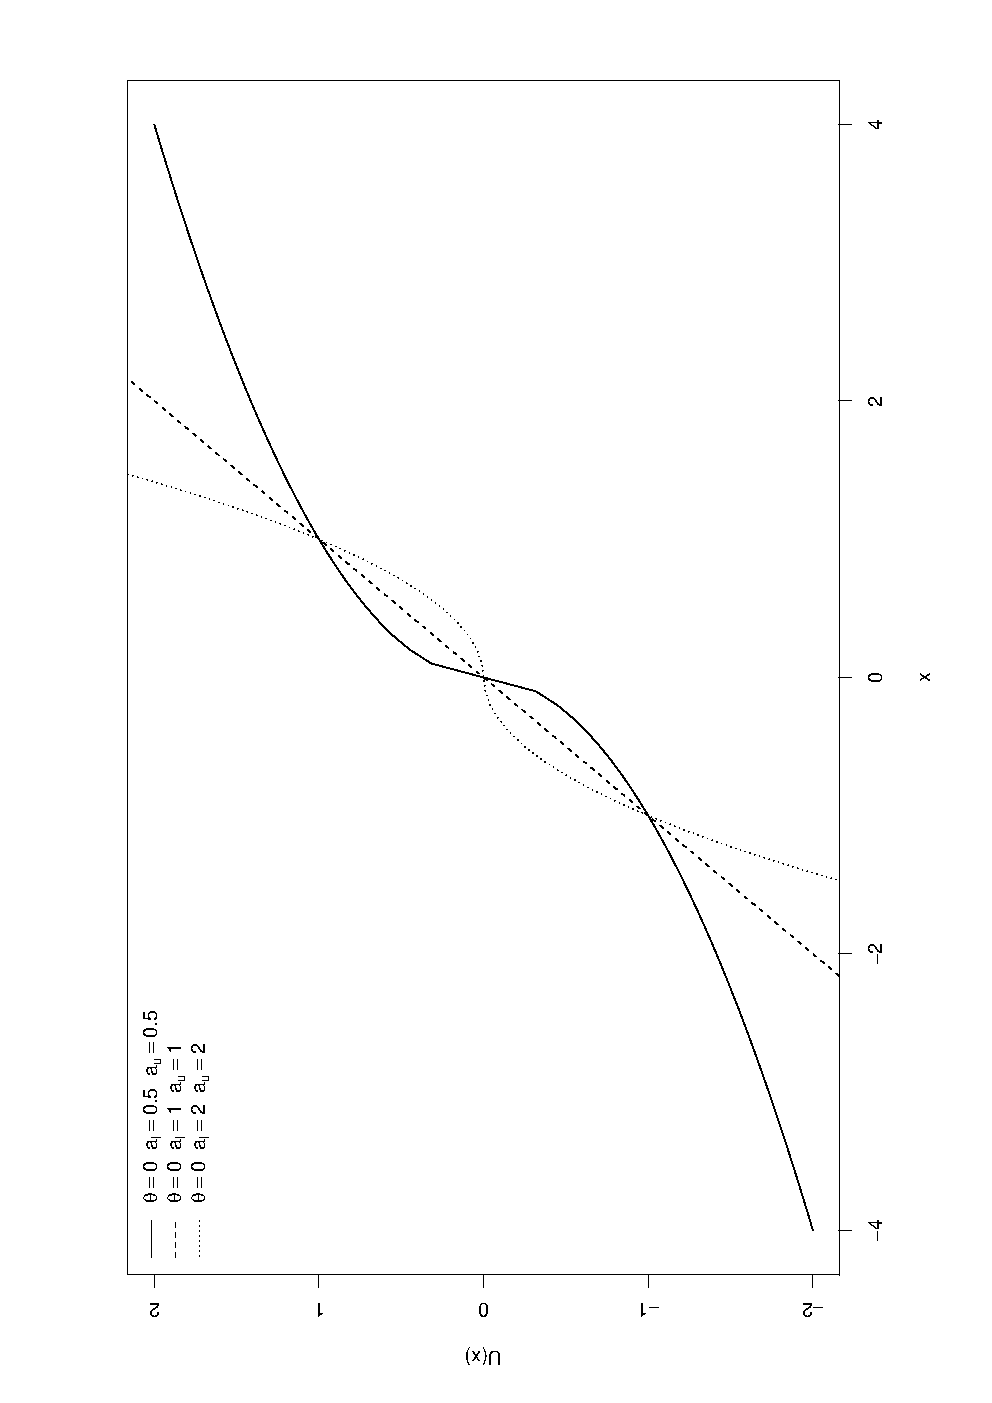
\includegraphics[scale=0.5,angle=-90,width=15cm]{lpmutility.png}
\caption[Upper to Lower Partial Moment Utility]{Upper to Lower Partial Moment Utility}\label{fig:lpmutility}
\end{figure} 
Unfortunately, this measure is non-convex and pretty hard to optimize with
confidence. At present the \textbf{parma} package experimentally supports
Global Optimization (GO) using a derivative free penalty function approach
and this model may be optimized under this setup (the \emph{LPMUPM} measure).
However, without making use of advanced state of the art commercial global
optimization solvers, it is quite hard to gauge the optimality of this solution
and the user should not expect too much as things currently stand.
\subsection{Conditional Value at Risk (CVaR)}\label{cvar}
Since the report by the Group of Thirty \citet{G301993}, the use of
Value  at Risk (VaR) is almost universal among banks, trading desks and other
financial entities as a key measure for measuring and managing risk. Despite
its popularity, it has come under growing pressure as a non coherent (it
lacks the subadditivity property) and inadequate measure, or an imperfect
measure which which has been incorrectly used, overused, abused and
over-relied upon. An alternative measure, based on the average loss
conditional on the VaR being violated is called Conditional Value at Risk
(CVaR)\footnote{Also called Expected Tail Loss with distinctions in the names
sometimes denoting differences for the continuous and sample cases, with the
latter requiring a specialized representation in order to be deemed convex
according to \citet{Rockafellar2000}.} which is a coherent and convex
risk measure belonging to the class of spectral risk measures of
\citet{Acerbi2002}. Formally, a spectral risk measure $M_\psi$ is a
weighted average of the the loss distribution quantile $q$ evaluated at $p$,
such that:
\begin{equation}
{M_\psi }=\int_0^1 {\psi \left( p \right){q_p}dp}
\end{equation}
where $\psi\left(p\right)$ is a weighting function defined over the full
range of  probabilities $p \in \left[ {0,1} \right]$ and restricted to be
non-negative, normalized to sum to 1, and increasing or constant in $p$ (such
that higher losses have equal or higher weights to lower loses). VaR is
clearly a spectral risk measure with weighting the dirac delta function which
is degenerate, while CVaR is based on a step function (constant weight for
losses greater than VaR). \citet{Cotter2006} investigated alternative
weighting functions to account for truly risk averse behavior by considering
strictly increasing weights functions in an application for establishing
futures clearinghouse margin requirements. While they found that such
weighting schemes were superior to the standard CVaR, \citet{Dowd2008}
also found some problems in their implementation both in the choice of
functions as well as the mixing properties of these measures with respect to
nonlinear weighting functions. In a different direction
\citet{Rockafellar2006} considered the so called mixed-CVaR problem
whereby it is possible to mix together CVaR at different coverage rates using
a weighting function, and established the relationship between this and the
spectral risk representation. In terms of the general optimization problem,
CVaR many be represented as an NLP minimization problem with objective
function given by:
\begin{equation}
\mathop {\min }\limits_{w,v} \frac{1}{na}\sum\limits_{i=1}^n {\left[ {\max \left( {0,v - \sum\limits_{j=1}^m {{w_j}{r_{i,j}}} } \right)} \right] - v}
\end{equation}
where $v$ is the $a$-quantile of the distribution. For a discrete scenario,
this can be represented using auxiliary variables as the following LP problem
(due to \citet{Rockafellar2000}):
\begin{equation}
\begin{gathered}
  \mathop {\min }\limits_{w,d,v} \frac{1}{{na}}\sum\limits_{i=1}^n {{d_i} + v}  \hfill \\
  s.t. \hfill \\
  \sum\limits_{j=1}^m {{w_j}{r_{i,j}} + v}  \geq  - {d_i},\forall i \in \left\{ {1,...,n} \right\} \hfill \\
  \sum\limits_{j=1}^m {{w_j}{\mu _j}=C}  \hfill \\
  \sum\limits_{j=1}^m {{w_j}=1}  \hfill \\
  {w_j} \geq 0,\forall j \in \left\{ {1,\dots,m} \right\} \hfill \\
  {d_i} \geq 0,\forall i \in \left\{ {1,\dots,n} \right\} \hfill \\
\end{gathered}
\end{equation}
where $v$ represents the VaR at the $a$-coverage rate and $d_i$ the
deviations  below the VaR. The formulation presented here is in such a way
as to represent the asset returns scenario matrix rather than the more typical
loss representation in the literature.\\
Direct extensions have followed in the same vein as the LPM measures with
\citet{Biglova2004} proposing the Rachev Ratio as the upper to lower
CVaR for which they provide a mixed integer representation in
\citet{Stoyanov2007} (modified by \citet{Konno2011} for cases when
the returns are completely distributed on the positive side), and also
proposed in the same paper the Generalized Rachev Ratio which is the Rachev
Ratio but with the numerator and denominator raised to different powers
representing different penalization to gains and losses beyond some upper and
lower quantiles. Unfortunately, this generalization, like the upper to lower
LPM has both a convex numerator and denominator\footnote{Technically, both
risk and reward CVaR functions are convex for values of the power $\ge 1$.}
making it non quasi-convex and hence necessitating a GO approach which will
be supported in due course.\footnote{The mixed-integer approach for the
Rachev Ratio is just as difficult to estimate as it is limited by the size of
the scenario which determines the number of binary variables required.}
\subsection{Conditional Drawdown at Risk (CDaR)}
Drawdown is an interesting concept in the literature on optimization since
this is a strongly path dependent measure. With the exception of Brownian
motion with zero drift discussed in \citet{Douady1999}, there is no
closed form solution for the distribution of this measure. While some
interesting solutions have been proposed, see for instance
\citet{Magdon-Ismail2004}, the measure considered here and its
optimization is based on \citet{Chekhlov2005}. The problem may be posed
as the following LP:
\begin{equation}
\begin{gathered}
  \mathop {\min }\limits_{w,u,v,z} v + \frac{1}{{na}}\sum\limits_{i=1}^n {{z_i}}  \hfill \\
  s.t. \hfill \\
  {z_i} - {u_i} + v \geqslant 0,\forall i \in \left\{ {1,\dots,n} \right\} \hfill \\
  \sum\limits_{j=1}^m {{w_j}{r_{i,j}} + {u_i} - {u_{i - 1}}}  \geqslant 0,{u_0}=0,\forall i \in \left\{ {1,\dots,n} \right\} \hfill \\
  {z_i} \geqslant 0,{u_i} \geqslant 0,\forall i \in \left\{ {1,\dots,n} \right\} \hfill \\
  \sum\limits_{j=1}^m {{w_j}{\mu _j}=C}  \hfill \\
  \sum\limits_{j=1}^m {{w_j}=1}  \hfill \\
  {w_j} \geqslant 0,\forall j \in \left\{ {1,\dots,m} \right\} \hfill \\
\end{gathered}
\end{equation}
where $z$ is an auxiliary vector of variables of the conditional drawdowns,
$u$ the auxiliary vector of variables to model the cumulative returns and
$v$ represents the Drawdown at Risk at the quantile level $a$. In the
\textbf{parma} package, this problem is represented only in LP form as of the
current release, allowing for both minimization subject to a minimum return
constraint or as an optimal risk-return fractional LP problem. In addition,
providing the type of scenario which makes sense in this context (i.e.
multi-period ahead) is completely left to the users' own devices, as it
remains a mystery to this author how to fully optimize multi-period
uncertainty in a single scenario and single-period SP setup.

\subsection{Comparison of Measures}\label{comparison}
The \emph{riskfun} function in the \textbf{parma} package provides a helpful utility
to investigate the properties of the risk/deviation measures discussed thus far. The
following table, taken from the first test example in the \emph{parma.tests} folder of the
package presents some insights into the properties of the risk measures:
{\tiny
\ctable[
pos = h,
cap     = {Properties of Risk/Deviation Measures.},
caption = {Properties of Risk/Deviation Measures.},
label   = {table:riskcompare},
center
]
{lcccccccc}
{
\tnote[]{\tiny {\bf Note:} The Table presents some of the properties of the measures used in the \textbf{parma} package,
where the definitions of the properties are defined in Section \ref{comparison}.
\LL}
}{
\FL
\begin{tabular*}{1\textwidth}{@{\extracolsep{\fill}}lcccccccc}
& \multicolumn{1}{c}{\boldmath{}\textbf{$MAD$}\unboldmath{}} & \multicolumn{1}{c}{\boldmath{}\textbf{$V$}\unboldmath{}} & \multicolumn{1}{c}{\boldmath{}\textbf{$SD$}\unboldmath{}} & \multicolumn{1}{c}{\boldmath{}\textbf{$MiniMax$}\unboldmath{}} & \multicolumn{1}{c}{\boldmath{}\textbf{$CVaR$}\unboldmath{}} & \multicolumn{1}{c}{\boldmath{}\textbf{$CDaR$}\unboldmath{}} & \multicolumn{1}{c}{\boldmath{}\textbf{$LPM_{m,\tau=c}$}\unboldmath{}} & \multicolumn{1}{c}{\boldmath{}\textbf{$LPM_{m,\tau=\mu}$}\unboldmath{}} \\
\boldmath{}\textbf{$Scaling$}\unboldmath{} & TRUE  & TRUE  & TRUE  & TRUE  & TRUE  & TRUE  & TRUE  & TRUE \\
\boldmath{}\textbf{$Location^{1}$}\unboldmath{} & TRUE  & TRUE  & TRUE  & FALSE & FALSE & FALSE & FALSE  & FALSE \\
\boldmath{}\textbf{$Location^{2}$}\unboldmath{} & FALSE & FALSE & FALSE & TRUE  & TRUE  & FALSE & TRUE & TRUE \\
\boldmath{}\textbf{$Subadditivity$}\unboldmath{} & TRUE  & FALSE & TRUE  & TRUE  & TRUE  & TRUE  & FALSE & TRUE \\
\end{tabular*}
\LL
}}

The properties tested are defined as follows:
\begin{itemize}
\item Scaling $f(bX)=\frac{1}{b}f(X)$
\item $Location^{1}$ $f(a+X)=f(X)$
\item $Location^{2}$ $f(a+X)=f(X)+a$
\item Subadditivity $f(X_1)+f(X_2)\ge f(X_1+X_2)$
\end{itemize}
where $f$ is some measure, $b$ a positive scalar and $a$ some constant $\in \mathbb{R}$.
The scaling property is shared by all measures, being a feature of their underlying constituent functions,
and a requirement for using fractional programming. The fact that $MAD$, $V$, and $SD$ are location
invariant ($Location^{1}$) is not surprising since they are deviation measures, which means that they
are calculated after centering. It is no surprise either that variance ($V$) is not subadditive since
the square function is known to be superadditive,  whilst standard deviation ($SD$) is subadditive. This has
certain implications for the fractional programming problem which leads to an optimal Sharpe ratio, even
though it is the variance which is minimized. The next 3 measures, $CVaR$, $CDaR$, and $LPM$ are not
deviation measures and as such are not location invariant, but do have the location property ($Location^{2}$),
with the exception of $CDaR$ which is path dependent. While the location and scaling of the $LPM$ measure was
discussed in Section \ref{LPM}, it is interesting to note that subadditivity is only present when
the threshold is equal to the portfolio mean\footnote{Equivalent to setting the threshold to 999 in
the \emph{parmaspec} options }, something also discussed in \citet{Brogan2005}.
\section{General Problem Formulation}\label{sec:3}
As was summarized in Table \ref{table:solvers}, the \textbf{parma} package
supports a variety of solvers, depending on the type of objective and
constraints. This section briefly outlines the general MILP, QP, NLP and GNLP
formulations used.
\subsection{MILP}
The MILP problem may be very generally represented as:
\begin{equation}\label{milp}
\begin{gathered}
  \mathop {\min }\limits_{{\mathbf{w}},\{\}} {\mathbf{Sw}} \hfill \\
  s.t. \hfill \\
  \dots \hfill \\
  {\mathbf{U}} \leq {\mathbf{Aw}} \leq {\mathbf{L}} \hfill \\
  {\mathbf{Cw}}={\mathbf{b}} \hfill \\
  {\mathbf{w'1}}=budget \hfill \\
  {\delta _i}w_i^{lower} \leq {w_i} \leq {\delta _i}w_i^{upper} \hfill \\
  {\mathbf{\delta '1}}=\# assets \hfill \\
  w_i^{lower} \leq {w_i} \leq w_i^{upper}\hfill \\
\end{gathered}
\end{equation}
given a vector of weights $\mathbf{w}$ of length $m$, where $\{\}$ denote any
additional parameters passed to (\dots) additional problem specific
constraints. The $k$ inequality constraints are stacked in a $k\times m$
$\mathbf{A}$ matrix with lower and upper bounds of length $k$ given by
$\mathbf{L}$ and $\mathbf{U}$ respectively. The general equality constraints
are stacked in the $l\times m$ $\mathbf{C}$ matrix with bounds of length $l$
given by $\mathbf{b}$, where the budget constraint is represented separately
for clarity. Custom inequality and equality matrices can be passed in the
\textbf{parmaspec} function via the \emph{ineq.mat} and \emph{eq.mat}
arguments with their corresponding bounds given by (\emph{ineq.LB},
\emph{ineq.UB}) and (\emph{eqB}) respectively. Optionally, a cardinality
constraint based on an 'in-between or out' formulation is represented by use
of $m$ binary variables $\mathbf{\delta}$. The use of cardinality constraints
is only allowed when the \emph{targetType} argument in the \textbf{parmaspec}
is 'minrisk' since the use of the fractional programming 'optimal' option and
the 'in-between or out' cardinality constraint formulation makes the problem
no longer LP (because of the fractional multiplier). Additionally, it is possible
to pass a benchmark series which is subtracted from the weighted returns for
benchmark relative optimization. In that case, it is usual to set the upper and
lower bounds to some positive and negative values representing the allowable
deviations from the benchmark weights, the budget to zero, so that the
resulting weights represent active bets on the benchmark, and the forecast and
target return as active values (i.e. in excess of the benchmark). Finally,
and currently only supported by the MILP type problems\footnote{This may be extended in
future to the NLP formulation.}, a vector of probabilities may also be passed
(which must sum to 1), giving different weights to each row of the scenario.

\subsection{NLP}
The NLP problem may be very generally represented as:
\begin{equation}\label{nlp}
\begin{gathered}
  \mathop {\min }\limits_{\mathbf{w}} f\left( {{\mathbf{w}},\dots} \right) \hfill \\
  s.t. \hfill \\
  g\left( {{\mathbf{w}},\dots} \right) \leq {\mathbf{0}} \hfill \\
  h\left( {{\mathbf{w}},\dots} \right)={\mathbf{0}} \hfill \\
  \left| {\mathbf{w}'} \right|{\mathbf{1}}=c \hfill \\
  w_i^{lower} \leq {w_i} \leq w_i^{upper} \hfill \\
\end{gathered}
\end{equation}
where $g\left( {{\mathbf{w}},\dots} \right)$ is the convex inequality
function returning a vector of length equal to the actual inequalities
evaluated, and $h\left( {{\mathbf{w}},\dots} \right)$ the affine equality
function returning a vector of length $l$ of the actual equalities evaluated.
In the \textbf{parma} package, custom inequalities and equalities can be
passed in the \textbf{parmaspec} function as list of functions (via the
\emph{ineqfun} and \emph{eqfun} arguments) but the user must also pass their
equivalent jacobian functions (via the \emph{ineqgrad} and \emph{eqgrad}
arguments). The absolute sum of weights may be used to control leverage ($c$)
when the weights are allowed to take on negative values, else this translates
to a simply sum of weights when the weights are all positive. As in the MILP
problem, benchmark relative optimization is possible (see the previous section
for details).

\subsection{QP}
The quadratic formulation, for use in the EV type problem of
\citet{Markowitz1952} may be represented as:
\begin{equation}\label{qp}
\begin{gathered}
  \mathop {\min }\limits_{\mathbf{w}} {\mathbf{w'Sw}} \hfill \\
  s.t. \hfill \\
  {\mathbf{U}} \leq {\mathbf{Aw}} \leq {\mathbf{L}} \hfill \\
  {\mathbf{Cw}}={\mathbf{b}} \hfill \\
  w_i^{lower} \leq {w_i} \leq w_i^{upper} \hfill \\
\end{gathered}
\end{equation}
where $\mathbf{S}$ is some positive definite covariance matrix, and
constraints as in the LP case in Equation \eqref{milp}. Benchmark relative
optimization is fully supported, and in this case a vector of the covariance
between the benchmark and the portfolio must be passed (via the \emph{benchmarkS}
option in the \emph{parmaspec} function), where the first value is the variance of
the benchmark, so that the resulting joint covariance matrix constructed by the
routine is:
\begin{equation}
{\Sigma _{b,r}} = \left( {\begin{array}{*{20}{c}}
  {\sigma _b^2}&{{\sigma _{\left\{ {b,r} \right\}}}} \\ 
  {{\sigma _{\left\{ {b,r} \right\}}}}&{{\Sigma _r}} 
\end{array}} \right)
\end{equation}
and the portfolio relative risk is then given by ${\left( { - 1,w} \right)^\prime }{\Sigma _{b,r}}\left( { - 1,w} \right)$.
The rest of the values should be passed as explained in the MILP section. The interested reader should 
consult for example \citet{Stoyanov2007} pp.412--414 for details of benchmark relative optimization in a QP setup.
\subsubsection{Optimal Portfolio}\label{qpopt}
The optimal portfolios admit one of 2 equivalent representations, depending on whether we are maximizing reward to risk:
\begin{equation}
\begin{gathered}
  \mathop {{\text{max}}}\limits_{{\mathbf{x}},t} {\text{ }}{\mathbf{x'}}{f_r} \hfill \\
  {\text{s.t.  }}{\left( { - t,{\mathbf{x}}} \right)^\prime }{\Sigma _{b,r}}\left( { - t,{\mathbf{x}}} \right) \leqslant 1 \hfill \\
  {\mathbf{x'1}} = t \hfill \\
  t{\mathbf{L}} \leqslant {\mathbf{Ax}} \leqslant t{\mathbf{U}} \hfill \\
  t \geqslant 0 \hfill \\ 
\end{gathered}
\end{equation}
or minimizing risk to reward:
\begin{equation}
\begin{gathered}
  \mathop {{\text{min}}}\limits_{{\mathbf{x}},t} {\text{ }}{\left( { - t,{\mathbf{x}}} \right)^\prime }{\Sigma _{b,r}}\left( { - t,{\mathbf{x}}} \right) \hfill \\
  {\text{s.t.  }}{\mathbf{x'}}{f_r} = 1 \hfill \\
  {\mathbf{x'1}} = t \hfill \\
  t{\mathbf{L}} \leqslant {\mathbf{Ax}} \leqslant t{\mathbf{U}} \hfill \\
  t \geqslant 0 \hfill \\ 
\end{gathered}
\end{equation}
where it is understood that $f_r$ is the returns forecast, and in the case of benchmark relative optimization, the returns forecast in excess of the benchmark forecast.
\subsection{SOCP}
A Second Order Cone Programming (\emph{SOCP}) problem has the following form:
\begin{equation}
\begin{array}{l}
{\text{minimize    }}c'x\\
{\text{subject to   }}\left\| {{A_i}x + {b_i}} \right\| \le {{c'}_i}x + {d_i},{\text{   i = 1,\dots,L}}\\
\end{array}
\end{equation}
where $\left\| {...} \right\|$ denotes the euclidean norm so that $\left\| x \right\| = \sqrt {x'x}$. Special cases include linear, quadratic and quadratically constrained quadratic problems, as well as a number of nonlinear and possible non-differentiable problems. While SOCP is a special case of Semi-Definite programming (\emph{SDP}) it is always more efficient to solve these problems using special purpose solvers rather than more general ones.
 
A special set of constraints based on p-norms can be represented using SOCP. Consider the following
p-norm inequality constraint:
\begin{equation}
{\left\| x \right\|_p} = {\left( {\sum\limits_{i = 1}^n {{{\left| {{x_i}} \right|}^p}} } \right)^{1/p}} \le t
\end{equation}
which involves the p-norm of a vector x $\in \Re^n$. We can re-write $p$ as $l/m$, where $l\ge m$, so that:
\begin{equation}
{\left\| x \right\|_p} = {\left( {\sum\limits_{i = 1}^n {{{\left| {{x_i}} \right|}^{l/m}}} } \right)^{m/l}} \le t
\end{equation}
and is equivalent to the following set of constraints:
\begin{equation}
\begin{array}{l}
 - {x_i} + {t^{\frac{{l - m}}{l}}}s_i^{\frac{m}{l}} \ge 0\\
{x_i} + {t^{\frac{{l - m}}{l}}}s_i^{\frac{m}{l}} \ge 0\\
{s_i} \ge 0,{\rm{  }}i = 1,...,n\\
\left( {\sum\limits_{i = 1}^n {{s_i}} } \right) \le t,{\rm{  }}t \ge 0
\end{array}
\end{equation}
where $s$ is an auxilliary vector of variables of same size as the original decision vector x. Obviously, the inequality can be turned into an equality using one extra constraint. However, care should be taken to allow for some slack between the upper and lower bounds of the 2 inequality constraints used to represent one equality else numerical difficulties may be encountered by the solver. It thus follows from the above type of exposition that it is quite easy to include a leverage constraint in a long/short portfolio optimization setting by setting $l=m=1$ which represents the manhattan norm.

In the parma package, problems which include the covariance matrix instead of a scenario may be solved either by the QP solver else the SOCP solver. In the latter case, there is a greater deal of flexibility since QCQP problems are easily solved (see the option for a list of matrices \emph{Q} in the documentation on \textbf{parmaspec}), as is the case of long/short optimization with a leverage (gross sum) constraint and the optimal risk to reward problem using the fractional approach of Section \ref{qpopt}


\subsection{GNLP}
The GNLP problem in the \textbf{parma} package is represented by use of
derivative free penalty functions as:
\begin{align}
\mathop{\min }\limits_{\mathbf{w}}f\left( {{\mathbf{w}},\dots} \right) & +
{p}\sum\limits_{i=1}^k {\max {{\left( {{g_i}\left( {{\mathbf{w}},\dots}
\right),0} \right)}^2}}\\ \nonumber
& + {p}\sum\limits_{i=1}^l {{h_i}{{\left( {{\mathbf{w}}, \ldots } \right)}^2}}
+ {p}\max {\left( {0,\sum\limits_{i=1}^m {{I_{\left| {{w_i}} \right| > 0.001}} - \# assets} } \right)^2}\\
&s.t.\hfill \\ \nonumber
&w_i^{lower} \leq {w_i} \leq w_i^{upper}\\ \nonumber
\end{align}
where $p$ is a penalty parameter. No gradients are used in this case which means that
any user specified equality and inequality functions can be passed (without Jacobians).
All NLP problems can be solved by GNLP, but mileage will vary with regards to the optimality
of the solution.

\section{Optimal Portfolios}\label{sec:4}
Consider the general nonlinear problem of minimizing a risk to reward problem represented as a fraction:
\begin{equation}\label{eq:fractional1}
\begin{gathered}
  \mathop {\min }\limits_{\mathbf{w}} \frac{{{\rho _{risk}}\left( {{\mathbf{Rw}}} \right)}}{{{\rho _{reward}}\left( {{\mathbf{Rw}}} \right)}} \hfill \\
  {\mathbf{w}}'{\mathbf{1}}=1 \hfill \\
  {\mathbf{L}} \leq {\mathbf{Aw}} \leq {\mathbf{U}} \hfill \\
  {\mathbf{w}} \geq 0 \hfill \\
\end{gathered}
\end{equation}
where $\mathbf{w}$ is an $m\times 1$ vector of weights, $\mathbf{R}$ the
$n\times m$ Scenario matrix of returns so that the risk ($\rho_{risk}$) and
reward ($\rho_{reward}$) functions are applied on the weighted scenario
returns, $\mathbf{1}$ an $m\times 1$  vector ones and $\mathbf{A}$ a $q\times
m$ matrix of linear constraints with lower and upper bounds given by
$\mathbf{L}$ and $\mathbf{U}$ respectively. The key developments in the
theory of fractional programming were provided in the linear case by
\citet{Charnes1962}, while for nonlinear cases the main contributions
can be traced to \citet{Dinkelbach1967} and
\citeauthor{Schaible1976a}(\citeyear{Schaible1976a},
\citeyear{Schaible1976b}). More recently, \citet{Stoyanov2007} provided
a more focused review of fractional programming with reference to financial
portfolio optimization. Under the assumption that both numerator and
denominator are positive homogeneous, the problem in \eqref{eq:fractional1}
can be transformed into the following simpler nonlinear fractional
programming (\emph{NLFP}) problem:
\begin{equation}\label{eq:fractional2}
\begin{gathered}
  \mathop {\min }\limits_{{\mathbf{\hat w}},\upsilon } {\rho _{risk}}\left( {{\mathbf{R\hat w}}} \right) \hfill \\
  {\rho _{reward}}\left( {{\mathbf{R\hat w}}} \right) \geq 1 \hfill \\
  {\mathbf{\hat w}}'{\mathbf{1}}=\upsilon  \hfill \\
  \upsilon {\mathbf{L}} \leq {\mathbf{A\hat w}} \leq \upsilon {\mathbf{U}} \hfill \\
  \upsilon  > 0 \hfill \\
\end{gathered}
\end{equation}
where $\upsilon$ represents a scalar auxiliary scaling variable and
$\mathbf{\hat w}$ the unconstrained optimal weight vector such that the
optimal weight vector $\mathbf{w}=\frac{\mathbf{\hat w}}{\upsilon}$. In order
for this problem to be convex, the reward function must be concave and the
risk function convex, with strict positivity required for both
functions.\footnote{For the reward function the requirement is a little more
relaxed in that there must be at least some combination of the weights and
returns for which the reward is positive. Additionally, for a linear reward
function the constraint becomes an equality.} Different relaxations of these
basic conditions lead to different classes of problems in the literature,
some with unique solutions and others requiring global search methods for
solution. These simple conditions admit both convex risk and deviation
measures as defined in Section \ref{sec:2}. The \textbf{parma} package
implements LP, QP and NLP based fractional optimization for all measures so
far discussed, including benchmark relative problems, and in the case of
the NLP formulation the analytical gradient of the functions and jacobian
of the constraints have also been derived and used.\footnote{This excludes
the case of cardinality constraints which make the problems non convex}
\section{Smooth Approximations to Non-Continuous Functions}\label{sec:5}
While it is preferable to work with an LP formulation of a decision problem,
there are certain situations where this poses certain challenges. First, for
some LP problems, the dimension of the dataset and constraints may tax the
limits of computer memory. Consider for example the MAD model presented in
Section \ref{sec:2} which has a constraint matrix of size $2n \times m$ in
order to create the piecewise linear representation for the absolute value,
where for large scenarios (n) and assets (m) memory considerations become
important. Second, in practise, many problems and/or constraints simply
cannot be expressed in LP form necessitating the use of either QP or NLP
based methods. In that case, it is always preferable to have analytic
derivatives of the function and constraints, for speed and accuracy versus
numerically evaluation methods. Interestingly, some problems, while convex
are discontinuous because of the presence of such functions as make use of
the \emph{minimum} or \emph{absolute} values. For these problems, an
approximation may be obtained by considering smooth and continuous versions
of these functions. Consider for example the CVaR and LPM measures, both of
which depend on the max function, for which the following smooth
approximation, $s_{max}$ may be used:
\begin{equation}\label{eq:smax}
\max \left( {x,0} \right) \approx {s_{\max }}\left( {x,0} \right)=\frac{{\left( {\sqrt {{x^2} + \varepsilon }  + x} \right)}}{2}
\end{equation}
where $\varepsilon$ is some very small positive number controlling the degree of approximation error. The absolute value may also be approximated
with the following function $s_{abs}$:
\begin{equation}\label{eq:sabs}
{abs} \left( {x} \right) \approx {s_{abs }}\left( {x} \right)=\sqrt {{{\left( {x + \varepsilon } \right)}^2}}
\end{equation}
although alternatives also exist\footnote{One such alternative is:  $\left(
{2x/\pi } \right)\left( {{{\tan }^{ - 1}}\left( {ox} \right)} \right)$, where
$o$ is some very large positive number.}. Apart from allowing the MAD problem
to be represented in NLP form with a smooth function, it also allows for the
use of short positions, replacing the full investment constraint with a
leverage constraint (the absolute sum of positions)\footnote{A common mistake
is to keep the full investment constraint instead of replacing it with the
leverage constraint, which makes no sense even when controlling for
individual position limits.}, without resorting to such methods as described
in \citet{Jacobs2006} which double the size of the problem and require
certain very specific assumptions about the 'trimability' of the portfolio.
Finally, for the case of the Minimax problem, it is possible to make use of
the generalized mean function ${M_p}\left( {{x_1},\dots,{x_n}} \right)={\left(
{\frac{1}{n}\sum\limits_{i=1}^n {x_i^p} } \right)^{1/p}}$, which
approximates the maximum of a set of positive values as $p \to  \infty$. In
order to obtain the maximum loss for use in the NLP minimax optimization
function, this function is combined with the $s_{max}$ function defined in
\eqref{eq:smax} applied to the negative of the scenario returns:
\begin{equation}\label{eq:sminimax}
{\left( {\frac{1}{n}\sum\limits_{i=1}^n {{s_{\max }}{{\left( { - {\mathbf{w}}'{\mathbf{r}_i},0} \right)}^p}} } \right)^{1/p}}.
\end{equation}
In practice, because the optimization problem needs to be calibrated for $p$,
making this a very hard problem, the \textbf{parma} package instead represents
the NLP objective in its LP form which leads to very high accuracy.
Table \ref{table:lpnlp1} shows the relative accuracy of the NLP representation of the
problems versus the exact LP formulation for a typical minimization problem, while
Table \ref{table:lpnlp2} shows the relative accuracy in a fractional problem setting.
{\tiny
\ctable[
pos = ht,
cap     = {LP vs NLP Smooth Approximations (minrisk)},
caption = {LP vs NLP Smooth Approximations (minrisk)},
label   = {table:lpnlp1},
center
]
{lcclcclcclcc}
{
\tnote[]{\tiny {\bf Note:} The Table reports the mean squared error (MSE), mean absolute error (MAE) and maximum error of the weights optimized
under the NLP smooth approximation representation versus the exact LP formulation. The absolute error (AbsErr) in the optimized
risk is also shown. The problem formulation was based on parma.test2 in the parma.tests folder of the \textbf{parma} package, using
the ETF dataset with the objective of minimizing risk given an equality for the target return.
\LL}
}{
\FL
\begin{tabular*}{1\textwidth}{@{\extracolsep{\fill}}lccccc}
      & \multicolumn{1}{c}{\textbf{MAD}} & \multicolumn{1}{c}{\textbf{MiniMax}} & \multicolumn{1}{c}{\textbf{CVaR}} & \multicolumn{1}{c}{\textbf{EV}} & \multicolumn{1}{c}{\textbf{LPM[1]}} \\
\textbf{MSE[weights]} & 4.18E-13 & 3.66E-31 & 4.53E-16 & 3.71E-18 & 2.10E-17 \\
\textbf{MAE[weights]} & 2.94E-07 & 2.81E-16 & 1.34E-08 & 1.03E-09 & 2.53E-09 \\
\textbf{MaxE[weights]} & 2.20E-06 & 1.78E-15 & 4.74E-08 & 5.63E-09 & 1.23E-08 \\
\textbf{AbsErr[risk]} & 1.37E-11 & 6.94E-17 & 2.04E-12 & 1.53E-08 & 1.85E-14 \\
\end{tabular*}
\LL
}}

{\tiny
\ctable[
pos = ht,
cap     = {LP vs NLP Smooth Approximations (fractional)},
caption = {LP vs NLP Smooth Approximations (fractional)},
label   = {table:lpnlp2},
center
]
{lcclcclcclcc}
{
\tnote[]{\tiny {\bf Note:} The Table reports the mean squared error (MSE), mean absolute error (MAE) and maximum error of the weights optimized
under the NLP smooth approximation representation versus the exact LP formulation. The absolute error (AbsErr) in the optimized
risk is also shown. The problem formulation was based on parma.test3 in the parma.tests folder of the \textbf{parma} package, using
the ETF dataset with the fractional objective of minimizing risk/reward.
\LL}
}{
\FL
\begin{tabular*}{1\textwidth}{@{\extracolsep{\fill}}lccccc}
      & \multicolumn{1}{c}{\textbf{MAD}} & \multicolumn{1}{c}{\textbf{MiniMax}} & \multicolumn{1}{c}{\textbf{CVaR}} & \multicolumn{1}{c}{\textbf{EV}} & \multicolumn{1}{c}{\textbf{LPM[1]}} \\
\textbf{MSE[weights]} & 5.35E-10 & 1.28E-35 & 1.34E-23 & 8.89E-19 & 1.25E-24 \\
\textbf{MAE[weights]} & 1.27E-05 & 9.51E-19 & 1.87E-12 & 4.57E-10 & 5.37E-13 \\
\textbf{MaxE[weights]} & 5.93E-05 & 1.39E-17 & 1.02E-11 & 2.71E-09 & 3.20E-12 \\
\textbf{Err[risk]} & 1.05E-07 & 6.94E-18 & 2.62E-12 & 1.91E-08 & 4.66E-15 \\
\end{tabular*}
\LL
}}

\section{Custom Constraints}\label{sec:6}
Since versions 1.5-0 the package has exported a number of custom constraint functions and their analytic derivatives (jacobians) to be used with NLP formulations. At present,
there are a set of functions for defining turnover constraints and a maximum portfolio variance given a user supplied covariance matrix. These functions can be passed to \emph{parmaspec} quite easily and details are provided in the documentation. This section will instead provide for a brief description of the type of turnover constraints which are included.
\subsection{Simple Turnover}
The simple turnover ($T$) constraint, given the set of optimal decision weights ($\mathbf{w}$) versus the existing set of weights ($\mathbf{w}^{old}$) can be represented as:
\begin{equation}
\sum\limits_{i = 1}^m {\left| {{w_i} - w_i^{old}} \right| \leqslant T,T \in {\mathbb{R}^ + }}
\end{equation}
Because of the absolute value function, this problem is most easily represented in an NLP setup with the use of the smooth absolute value function presented in Section \ref{sec:5}. For LP problems, this may also be formulated by use of auxiliary variables and this may be included in the package at a future time.
\subsection{Buy and Sell Turnover}
A more flexible turnover constraint limits the buy ($T^+$) and sell ($T^-$) turnover separately, and can be represented as:
\begin{equation}
\begin{gathered}
  \sum\limits_{i = 1}^m {\max \left( {0,{w_i} - w_i^{old}} \right) \leqslant {T^ + },{T^ + } \in {\mathbb{R}^ + }}  \hfill \\
  \sum\limits_{i = 1}^m {\max \left( {0,w_i^{old} - {w_i}} \right) \leqslant {T^ - },{T^ - } \in {\mathbb{R}^ + }}  \hfill \\
\end{gathered}
\end{equation}
where again the smooth approximation to the maximum value function presented in Section \ref{sec:5} is used. \textbf{When using this
constraint in a fractional programming setup, care should be taken that the combination of bounds, turnover limits and the forecast return
vector do not result in a negative expected return in which case the problem is not solvable}.

\section{FAQ's and Misc Notes}\label{sec:7}
The following additional notes may be of interest:
\begin{itemize}
\item QCQP (Quadratically Constrained Quadratic Problems) are not yet
    implemented but may be in due course.
\item Custom equality constraints in NLP problems MUST be affine in order
    to  guarantee convexity of the problem.
\item Custom inequality constraints in NLP problems MUST be convex in
    order to  guarantee convexity of the problem.
\item No plots yet...may come in due course.
\item The parma.tests folder (under the \emph{inst} folder in the source)
    contains a large number of instructive examples.
\end{itemize}
If you have questions, use the R-SIG-FINANCE mailing list to ask them.\\ 
\clearpage
\bibliography{parmabib}
\end{document}
